\section{Evaluation}
\label{sec:experiments}

The evaluation is organized by substrate rather than by historical run name.
It reports what the current artifacts support and what they do not support.
All public final-text source-mismatch accepts below are spoofing evidence only;
they are not protected success, not codeword recovery, and not public
text-only verification.

\subsection{Trace-Bound Controllability}
\label{subsec:trace-bound-results}

The trace-bound diagnostic tests provider-side first-divergence event access.
Table~\ref{tab:trace-bound-results} reports protected recovery and the four
control arms.

\begin{table}[t]
\centering
\small
\setlength{\tabcolsep}{4pt}
\begin{tabular}{lccccc}
\toprule
Model & Protected & Raw & Task-only & Wrong-key & Wrong-payload \\
\midrule
Qwen & 94/96 & 0/96 & 0/96 & 0/96 & 0/96 \\
Llama & 96/96 & 0/96 & 0/96 & 0/96 & 0/96 \\
\bottomrule
\end{tabular}
\caption{Trace-bound first-divergence diagnostic results.  These numbers
support provider-side event controllability under trace access.  They do not
support public final-text-only verification success or an ownership proof.}
\label{tab:trace-bound-results}
\end{table}

The protected recovery rates show that the event-access substrate can carry a
recoverable codeword under reviewed controls.  The clean control arms rule out
the simplest raw, task-only, wrong-key, and wrong-payload explanations in this
diagnostic.  The result is deliberately scoped to trace-bound provider-side
access.

\begin{figure}[t]
\centering
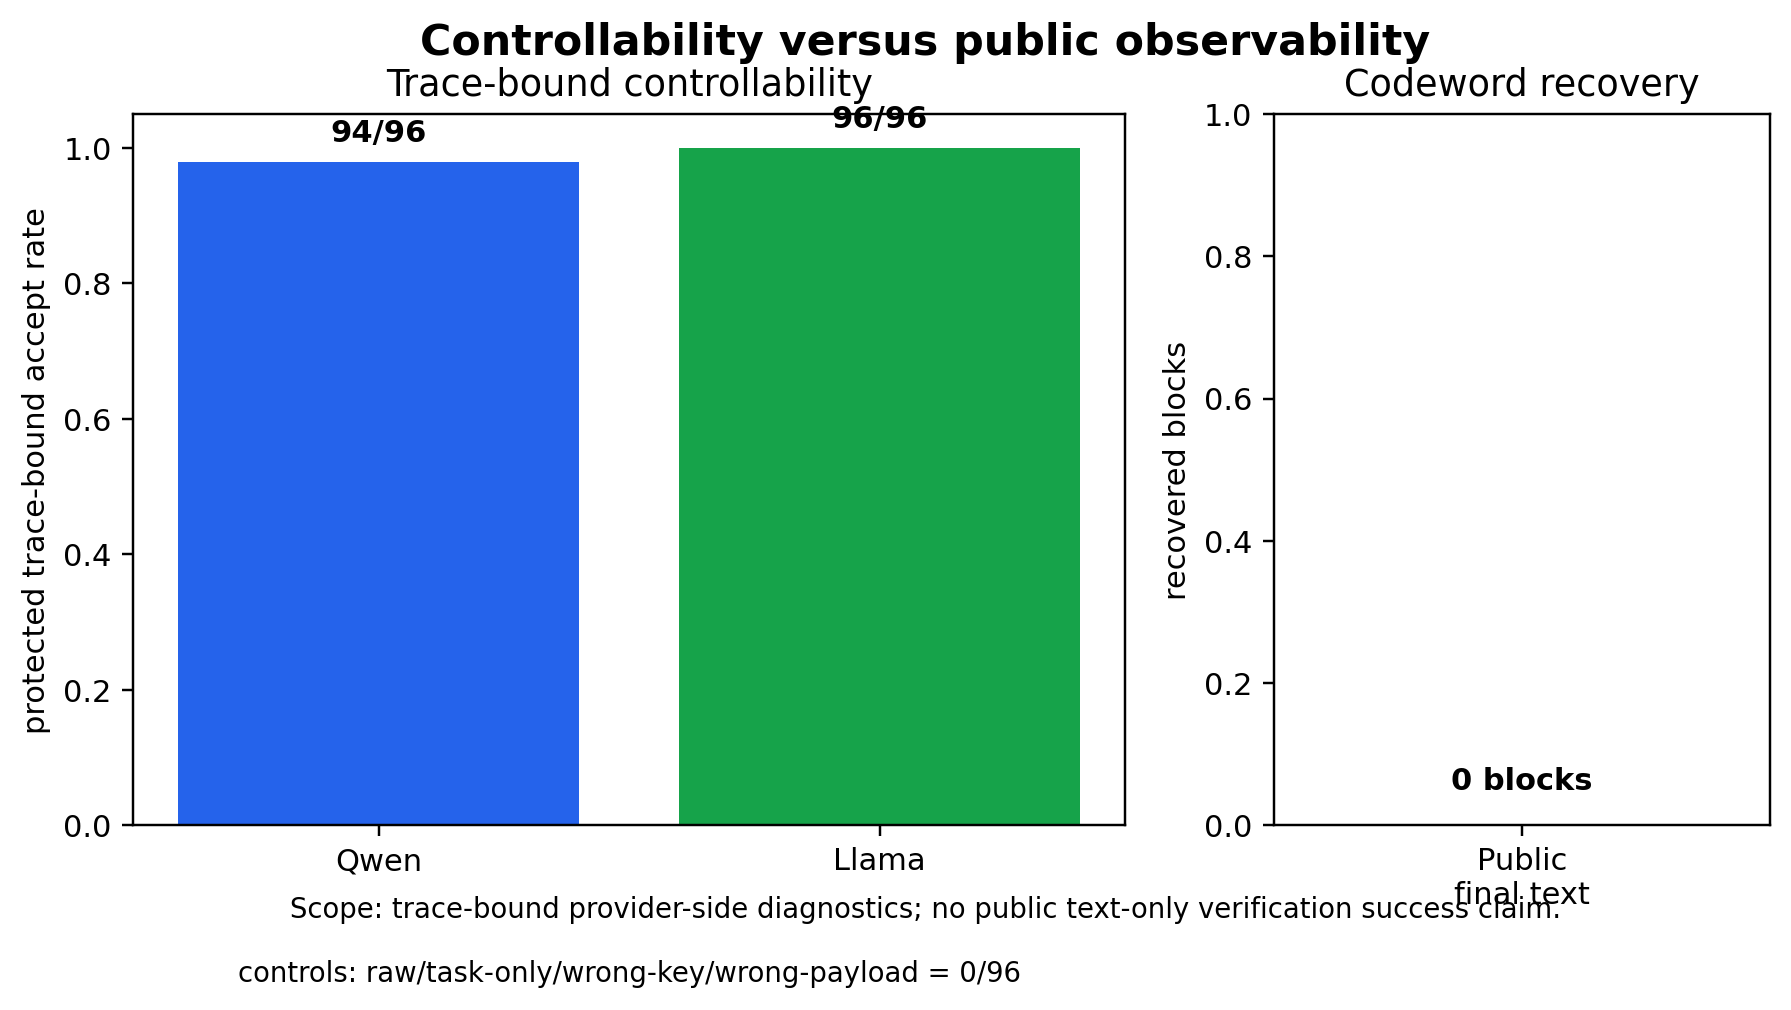
\includegraphics[width=\linewidth]{figures/figure_3_controllability_vs_observability.png}
\caption{Controllability versus public observability.  Trace-bound protected
accepts are high with clean controls, while public final-text codeword recovery
is not observed.  The figure supports a substrate-gap diagnosis, not public
text-only verification success.}
\label{fig:controllability-observability}
\end{figure}

\subsection{Public Final-Text Observability}
\label{subsec:public-text-results}

The public final-text route removes event access.  Across the current public
predicate artifacts, the number of recovered codeword blocks is zero.  The P2
predicates show shallow separability, summarized in
Table~\ref{tab:public-text-p2}, but no deterministic codeword recovery.

\begin{table}[t]
\centering
\small
\setlength{\tabcolsep}{4pt}
\begin{tabular}{lccccc}
\toprule
Model & AUC & Protected TPR & Raw FPR & Task-only FPR & Codeword blocks \\
\midrule
Qwen & 0.554676 & 0.275476 & 0.193455 & 0.195060 & 0 \\
Llama & 0.631280 & 0.154992 & 0.038798 & -- & 0 \\
\bottomrule
\end{tabular}
\caption{Public final-text P2 predicate diagnostics.  The predicates show
some protected/raw separability, but codeword recovery remains zero.  AUC is
not deterministic verification.}
\label{tab:public-text-p2}
\end{table}

This result is the core observability gap.  The trace-bound signal does not
become a public final-text codeword.  A public predicate can separate
distributions without verifying provenance.

\subsection{Public-Predicate Spoofing}
\label{subsec:attack-results}

The attack ladder evaluates whether source-mismatch rows can enter the public
predicate's accept region.  Table~\ref{tab:attack-ladder} summarizes rejection
sampling, distillation-lite ranking, and guided rewrite/graft.

\begin{table}[t]
\centering
\scriptsize
\setlength{\tabcolsep}{3pt}
\begin{tabular}{llccc}
\toprule
Source & Arm & Rejection top-100 & Distillation top-100 & Guided top-100 \\
\midrule
Qwen & raw & 14/100 & 51/100 & 100/100 \\
Qwen & task-only & 20/100 & 38/100 & 100/100 \\
Llama & raw & 5/100 & 20/100 & 100/100 \\
\bottomrule
\end{tabular}
\caption{Public-predicate attack ladder on source-mismatch rows.  Guided
rewrite/graft reaches 100/100 accepted top-ranked examples for all three
listed source arms, at 3,400 predicate queries per top-100 source set.  These
are source-mismatch spoofing examples, not protected success.}
\label{tab:attack-ladder}
\end{table}

Rewrite-lite also produces thousands of new source-mismatch accepts under
deterministic opener edits: 6,232 prepend-opener and 7,108 replace-opener new
accepts for Qwen raw; 6,214 and 6,957 for Qwen task-only; and 7,973 and 9,384
for Llama raw.  Distillation-lite enriches top-ranked source-mismatch accepts:
Qwen raw reaches 51/100 with 2.318x enrichment, Qwen task-only reaches 38/100
with 2.533x enrichment, and Llama raw reaches 20/100 with 20.0x enrichment.

The interpretation is narrow but important.  These attacks do not show
protected recovery.  They show that public final-text predicates with nonzero
accept regions are optimization targets.

\begin{figure}[t]
\centering
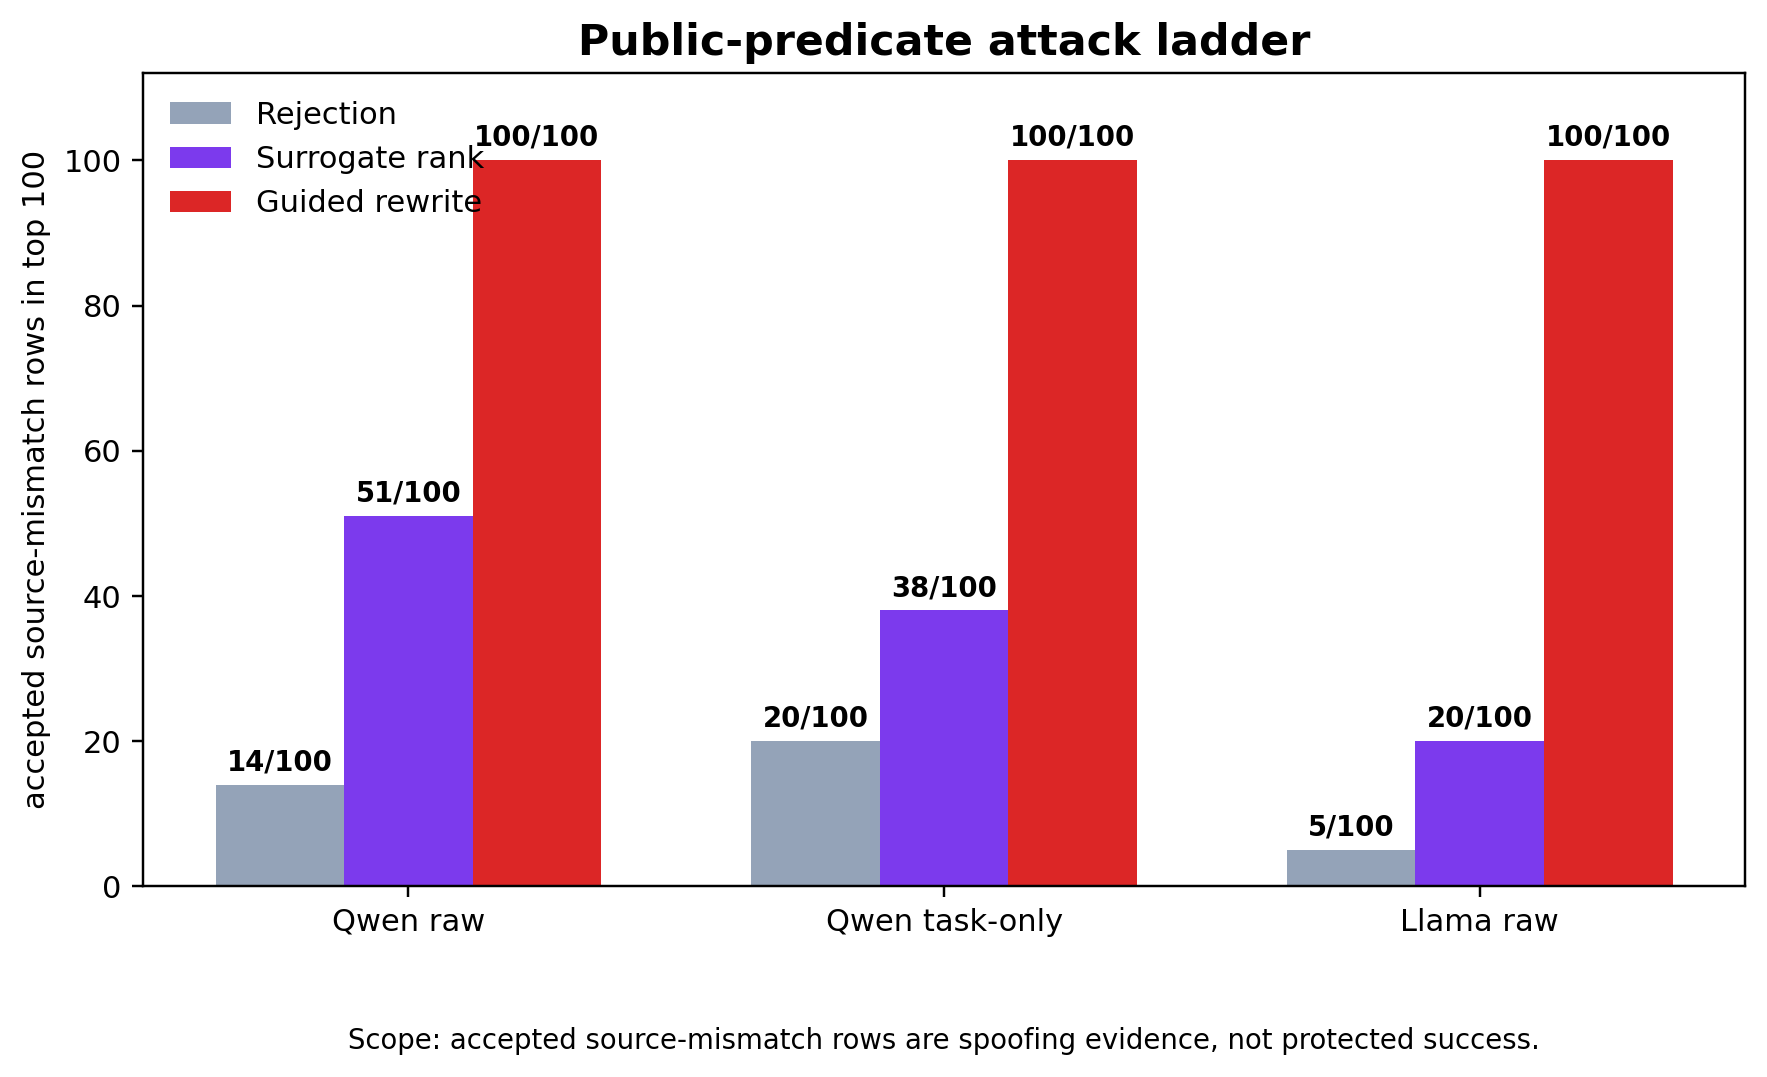
\includegraphics[width=\linewidth]{figures/figure_4_public_predicate_attack_ladder.png}
\caption{Public-predicate attack ladder.  Accepted rows in this figure are
source-mismatch spoofing examples produced under public predicate feedback.
They are not protected success, not codeword recovery, and not public
text-only verification.}
\label{fig:attack-ladder}
\end{figure}

\subsection{Template Leakage and Duplicate Quality}
\label{subsec:quality-results}

Earlier natural-output routes exposed quality problems that matter for the
substrate claim.  The template leakage audit reports Qwen shallow AUC 0.554676,
which passes the 0.60 gate, but a format-scrub duplicate extra row remains.
Llama reports shallow AUC 0.63128, which fails the 0.60 leakage gate.  These
quality failures are not repaired into positives.  They are evidence that final
text can carry visible or brittle regularities without becoming a reliable
verification substrate.

\subsection{Ownership Scenario Stress Test}
\label{subsec:ownership-stress}

The scenario stress test crosses seven ownership scenarios with nine method
families, for 63 cells.  The only currently supported scenario is the
cooperative provider with trace bundle.  The public final-text-only portable
supported set is empty.  This result is not a survey claim about all future
methods; it is a claim-boundary check for the current artifacts.

\begin{table}[t]
\centering
\small
\setlength{\tabcolsep}{4pt}
\begin{tabular}{lc}
\toprule
Stress-test quantity & Current value \\
\midrule
Scenario-method cells & 63 \\
Supported trace-bound scenarios & 1 \\
Supported public final-text-only portable scenarios & 0 \\
Supported scenario label & Cooperative provider with trace bundle \\
\bottomrule
\end{tabular}
\caption{Ownership scenario stress-test summary.  Current artifacts support a
cooperative trace-bundle diagnostic only.}
\label{tab:ownership-stress}
\end{table}

\begin{figure}[t]
\centering
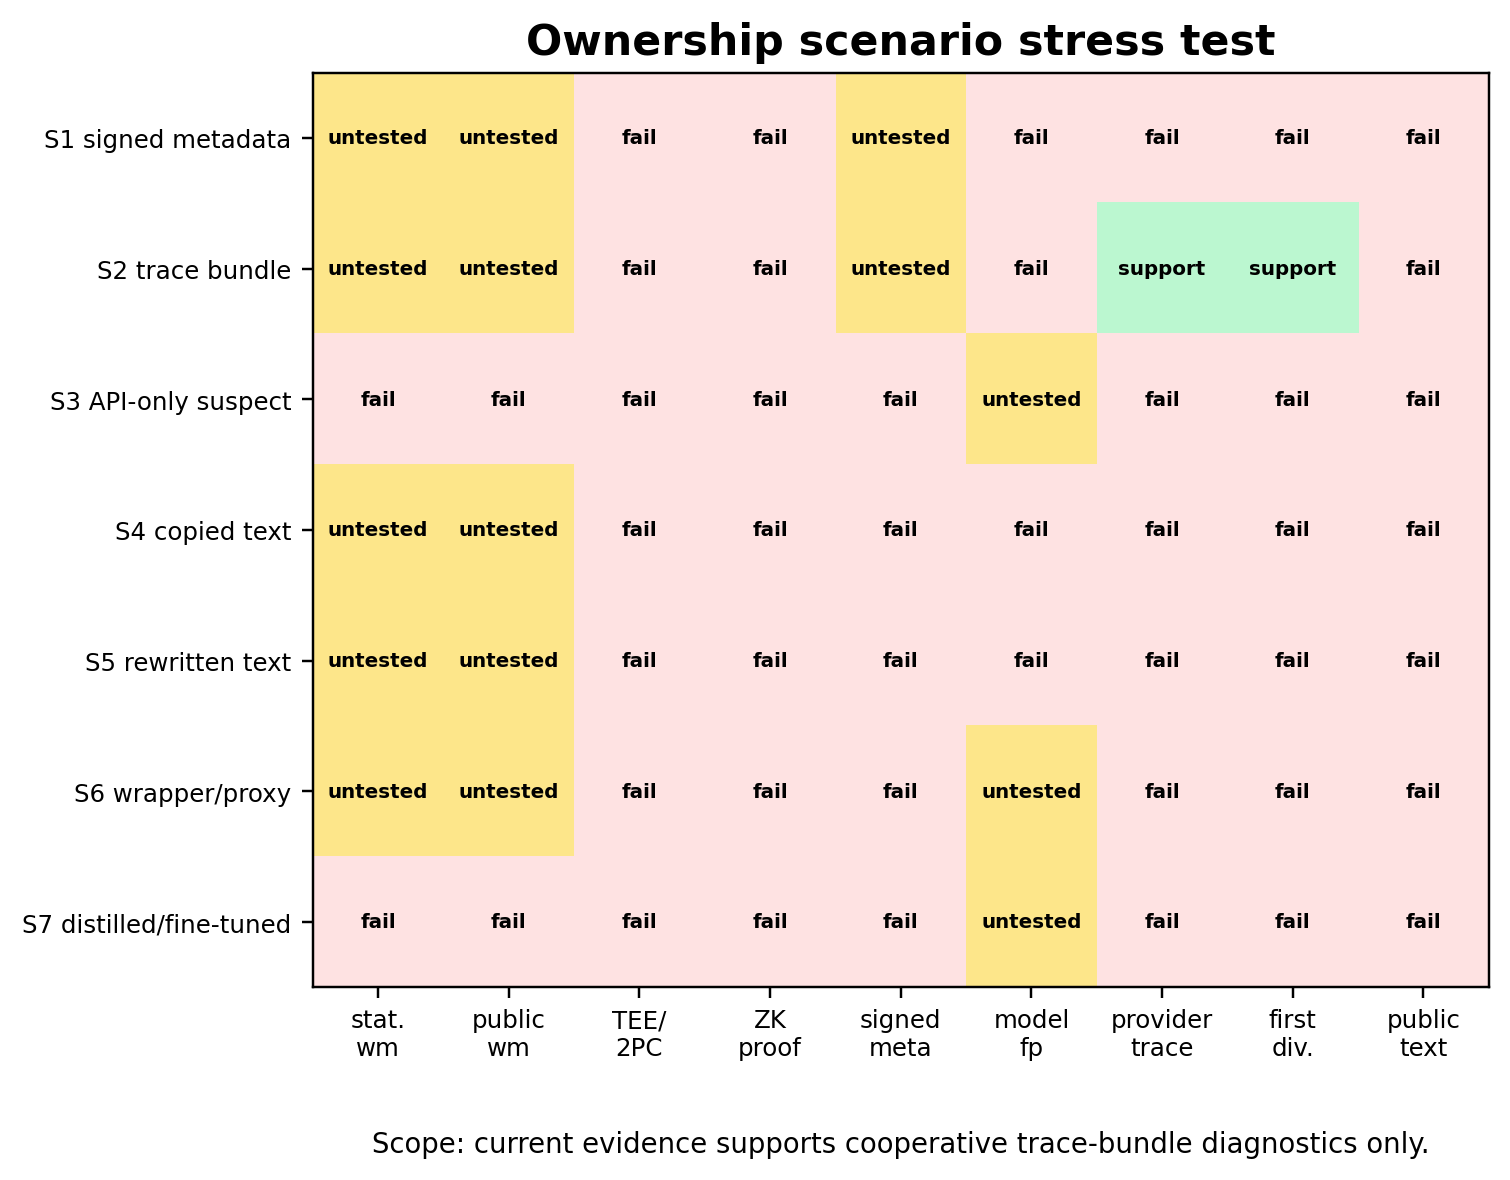
\includegraphics[width=\linewidth]{figures/figure_5_ownership_scenario_heatmap.png}
\caption{Ownership scenario heatmap.  The current artifacts support only the
cooperative provider trace-bundle diagnostic scenario; no public
final-text-only portable success scenario is supported, and no ownership proof
is claimed.  This is not public text-only verification success and not an
ownership proof.}
\label{fig:ownership-heatmap}
\end{figure}

\FloatBarrier
